\documentclass[tikz, border=15pt]{standalone}
\usepackage{tikz}
\usepackage{amsmath}
\usetikzlibrary{arrows.meta, calc, intersections, positioning}

\begin{document}
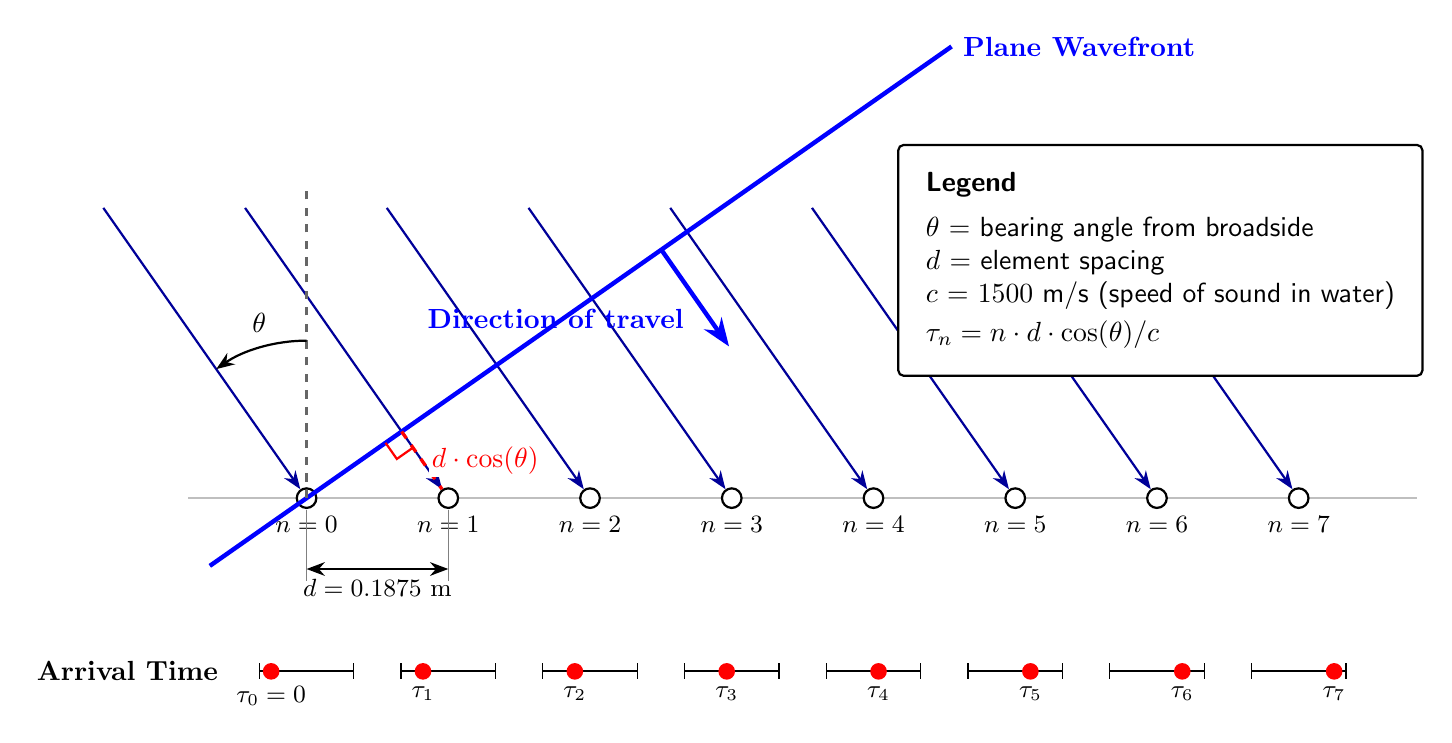
\begin{tikzpicture}[
font=\sffamily,
>=Stealth,
ray/.style={thick, blue!60!black, <-},
wavefront/.style={ultra thick, blue},
pathdiff/.style={very thick, red, dashed}
]

% ─── PARAMETERS ────────────────────────────────────────────────────────
\def\N{7}                        % Last element index (0 to 7 = 8 elements)
\def\d{1.8}                      % Element spacing
\def\thetaAngle{35}              % Bearing angle from broadside (degrees)

% Calculations based on broadside = 90 degrees (vertical)
\pgfmathsetmacro{\srcAngle}{90 + \thetaAngle}   % Angle to source = 125 deg
\pgfmathsetmacro{\propAngle}{\srcAngle - 180}   % Propagation direction = -55 deg
\pgfmathsetmacro{\wfAngle}{\propAngle + 90}     % Wavefront angle = 35 deg

% ─── 1. ARRAY AXIS & ELEMENTS ──────────────────────────────────────────
% Array baseline
\draw[thick, gray!50] (-1.5, 0) -- (\N*\d + 1.5, 0);

% Elements
\foreach \n in {0,...,\N} {
\node[circle, draw=black, fill=white, inner sep=2.5pt, thick] (E\n) at (\n*\d, 0) {};
\node[below=3pt, font=\small] at (E\n) {$n=\n$};
}

% Element spacing label (placed below to avoid intersecting rays)
\draw[thin, gray] (0, -0.15) -- (0, -1.05);
\draw[thin, gray] (\d, -0.15) -- (\d, -1.05);
\draw[<->, thick] (0, -0.9) -- (\d, -0.9) node[midway, below, font=\small] {$d = 0.1875\text{ m}$};

% ─── 2. INCIDENT RAYS ──────────────────────────────────────────────────
\foreach \n in {0,...,\N} {
\draw[ray] (E\n) -- ++(\srcAngle:4.5);
}

% ─── 3. WAVEFRONT ──────────────────────────────────────────────────────
% Draw the plane wavefront passing exactly through element 0
\coordinate (WF_start) at (\wfAngle + 180 : 1.5);
\coordinate (WF_end)   at (\wfAngle : 10);
\draw[wavefront] (WF_start) -- (WF_end) node[right, font=\bfseries] {Plane Wavefront};

% Direction of travel arrow
\coordinate (WF_mid) at (\wfAngle : 5.5);
\draw[ultra thick, blue, ->] (WF_mid) -- ++(\propAngle:1.5) 
node[midway, below left, font=\bfseries] {Direction of travel};

% ─── 4. PATH LENGTH DIFFERENCE (RIGHT TRIANGLE) ────────────────────────
% Calculate intersection of wavefront and the ray connecting to Element 1
% Since element 1 is at (\d, 0), the projection onto the wavefront is \d * \cos(\theta)
\coordinate (P) at (\wfAngle : {\d * cos(\thetaAngle)});

% Draw the extra path length as a red dashed line
% (Visually forms a vertical/orthogonal drop from the wavefront to the element)
\draw[pathdiff] (P) -- (E1) 
node[midway, right, xshift=2pt, fill=white, inner sep=1pt] {$d \cdot \cos(\theta)$};

% Right angle marker at P
\coordinate (P1) at ($ (P) ! 0.25cm ! (E0) $);
\coordinate (P3) at ($ (P) ! 0.25cm ! (E1) $);
\coordinate (P2) at ($ (P1) + (P3) - (P) $);
\draw[thick, red] (P1) -- (P2) -- (P3);

% ─── 5. BROADSIDE AND BEARING ANGLE ────────────────────────────────────
% Broadside vertical line
\draw[dashed, thick, gray!80!black] (0,0) -- (0, 4) coordinate (Broadside);

% Bearing angle \theta arc
\draw[thick, ->] (0, 2) arc (90:\srcAngle:2) 
node[midway, above=2pt] {$\theta$};

% ─── 6. TIME AXIS BELOW EACH ELEMENT ───────────────────────────────────
\node[left, font=\bfseries] at (-1.0, -2.2) {Arrival Time};

\foreach \n in {0,...,\N} {
\coordinate (TA) at (\n*\d, -2.2);

% Axis line and end ticks
\draw[thick] ($ (TA) + (-0.6, 0) $) -- ($ (TA) + (0.6, 0) $);
\draw[thin]  ($ (TA) + (-0.6, 0.1) $) -- ($ (TA) + (-0.6, -0.1) $);
\draw[thin]  ($ (TA) + (0.6, 0.1) $) -- ($ (TA) + (0.6, -0.1) $);

% Calculate progressive dot offset
\pgfmathsetmacro{\dotOffset}{-0.45 + \n*(0.9/\N)}

% Red dot representing arrival time \tau_n
\fill[red] ($ (TA) + (\dotOffset, 0) $) circle (3pt);

% Label \tau_n
\ifnum\n=0
\node[below=2pt, font=\small] at ($ (TA) + (\dotOffset, 0) $) {$\tau_0=0$};
\else
\node[below=2pt, font=\small] at ($ (TA) + (\dotOffset, 0) $) {$\tau_\n$};
\fi
}

% ─── 7. LEGEND BOX ─────────────────────────────────────────────────────
\node[draw=black, thick, fill=white, anchor=north west, align=left, 
inner sep=10pt, rounded corners=2pt] at (7.5, 4.5) {
\textbf{Legend} \\[4pt]
$\theta$ = bearing angle from broadside \\
$d$ = element spacing \\
$c$ = $1500\text{ m/s}$ (speed of sound in water) \\[2pt]
$\tau_n = n \cdot d \cdot \cos(\theta) / c$ 
};

\end{tikzpicture}
\end{document}